\section{Propagation models}
The calculation of the power density $S_R$ at the receiver at a given distance d can be done according to \autoref{eq:power_density}, where P is the power and $G_T$ the antenna gain.
\begin{equation}\label{eq:power_density}
    S_R=\frac{P \cdot G_T}{4 \pi d^2}
\end{equation}
The pointing vector can be calculated according to \autoref{eq:pointing_vector}
\begin{equation}\label{eq:pointing_vector}
    \vec{S}=\vec{E} \times \vec{H}
\end{equation}
The field wave impedance can be calculated according to \autoref{eq:field wave impedance}
\begin{equation}\label{eq:field wave impedance}
    Z_f=\frac{E}{H}=120 \pi \approx 377[\Omega]
\end{equation}
The Electrical field strength (rms) can be calculated according to \autoref{eq:electrical_filed_strength}, which as the combination of \autoref{eq:field wave impedance}, \autoref{eq:pointing_vector} and \autoref{eq:power_density}.
\begin{equation}\label{eq:electrical_filed_strength}
E=\sqrt{\frac{P \cdot G_T \cdot Z_f}{4 \pi d^2}}
\end{equation}
The equivalent absorption area of a receiving antenna is given by \autoref{eq:equivalen_absorption}
\begin{equation}\label{eq:equivalen_absorption}
    A_R=G_R \cdot \frac{\lambda^2}{4 \pi}
\end{equation}
\begin{equation}
P_R=\frac{P_T \cdot G_T \cdot G_R}{(4 \pi \cdot d / \lambda)^2}
\end{equation}
\autoref{eq:free_space_loss} Shows the free space loss:
\begin{equation}\label{eq:free_space_loss}
A_F=(4 \pi \cdot d / \lambda)^2
\end{equation}
Where $\lambda=\frac{\mathrm{V}}{\mathrm{f}}$.
\subsubsection{Wave propagation model by Okumura-Hata}
\begin{equation}\label{eq:okumura-hata}
L_{H u}[d B]=69.55+26.16 \cdot \log \frac{f}{M H z}-13.82 \cdot \log \frac{h_{B S}}{m}-a\left(h_{M S}\right)+\left(44.9-6.55 \log \frac{h_{B S}}{m}\right) \cdot \log \frac{d}{k m}
\end{equation}
\begin{itemize}
    \item Transmit frequency: $f$
    \item Height of base station antenna: $h_{BS}$
    \item Height of mobile station antenna: $h_{MS}$
    \item Distance: $d$
\end{itemize}
Correction terms
\begin{itemize}
    \item Correction term for small and medium-sized cities:
    $$
    a\left(h_{M S}\right)=\left(1.1 \cdot \log \frac{f}{M H z}-0.7\right) \cdot \frac{h_{M S}}{m}-\left(1.56 \cdot \log \frac{f}{M H z}-0.8\right)
    $$
    \item Correction term for metropolises:
    $$
    a\left(h_{M S}\right)= \begin{cases}8.29 \cdot\left[\log \left(1.54 \cdot \frac{h_{M S}}{m}\right)\right]_2^2-1.1 & f \leqslant 200 \mathrm{MHz} \\ 3.2 \cdot\left[\log \left(11.75 \cdot \frac{h_{M S}}{m}\right)\right]^2-4.97 & f \geqslant 400 \mathrm{MHz}\end{cases}
    $$
    \item Correction term for sub-urban areas:
    $$
    L_{H s}[d B]=L_{H u}-2 \cdot\left[\log \frac{f}{28 \mathrm{MHz}}\right]^2-5.4
    $$
    \item Correction term for rural areas:
    $$
    L_{H r}[d B]=L_{H u}-4.78 \cdot\left[ \log \frac{f}{M H z}\right]^2+18.33 \cdot \log \frac{f}{M H z}-40.94
    $$
\end{itemize}




\subsubsection{Air refraction effects}
Due to variations of air temperature/pressure/humidity, the refraction index varies with height above ground.
\subsubsection{Important radio channel effects in mobile communicaionts}
$$
\begin{array}{|c|c|}
\hline \text { Type/Reason } & \text { Effect } \\
\hline \text { Multipath } & \text { Fast Fading } \\
& \text { Delay Spread (Zeitdispersion) } \\
\hline \text { Movement } & \text { Doppler Shift } \\
& \text { Frequency Dispersion } \\
\hline \text { Shadowing effect } & \text { Slow Fading } \\
\hline \text { Path losses } & \text { Signal attenuation } \\
\hline
\end{array}
$$
The Doppler frequency is described with \autoref{eq:doppler_frequency}
\begin{equation}\label{eq:doppler_frequency}
f_D=\frac{1}{2 \pi} \frac{d \varphi}{d t}=f_m \sin \alpha
\end{equation}
The maximum Doppler frequency $f_m$ is given by 
\begin{equation}
f_m=\frac{v}{\lambda}=\frac{v}{c \cdot f}
\end{equation}

\subsubsection{coherence time and coherence bandwidth}
\begin{itemize}
    \item Coherence Time: measure for the time period in which the channel properties remain approximately constant.
    \begin{equation}\label{eq:corherence_time}
    \mathrm{T}_{\mathrm{tc}}=1 / \mathrm{B_d}
    \end{equation}
    $B_d$ = Doppler spread bandwidth
    \item Coherence bandwidth: measure for the bandwidth, in which the channel properties remain highly correlated.
    \begin{equation}\label{eq:coherence_bandwidth}
    \mathrm{B}_{\mathrm{cb}}=1 / \mathrm{T_m}
    \end{equation}
    $T_m$ = delay spread \newline
    $\Rightarrow$ all frequency component within $B_{cb}$ will be almost equally attenuated.
\end{itemize}

\paragraph{Two-ray-model}
A base station transceiver transmits a GSM signal on a channel within the frequency range of f = 935,2MHz...935.4MHz. A mobile station (MS) is connected to this base station (BS). Let us assume that there is a line-of sight condition between them. Imagine further that there is a mountain chain parallel to the line-of-sight connection at a distance of h=2km, which partially reflects incident radio signals.
Let us assume further:
\begin{enumerate}
    \item The mountain chain is modelled as a vertical wall (see figure below).
    \item The antennas of both the BS and the MS have an omnidirectional radiation pattern in the horizontal plane
    \item The radio signal propagates from the BS to the MS by just two paths, namely the direct path (i.e. line-of-sight), and one reflected path, by reflection at the vertical wall. (Any further reflections such as ground reflection shall be neglected).
    \item The reflection itself obeys the principles of geometrical optics.
    \item The attenuation of the receiving field strength due to the detour of the reflected path is neglected, or considered to be already included in the reflection coefficient \textcolor{orange}{r}.
    \item Distance between BS and MS: d = 5km
    \item Reflection coefficient at the wall for the E field under the given incident angle: r = 0.5 (real)
\end{enumerate}
\begin{itemize}
    \item \textbf{Determine the radio channel's amplitude response between the BS and the MS for the given GSM-channel (i.e. between 935,2 MHz ... 935,4 MHz)}\newline
    According to \autoref{eq:superimposed_complex_signal} the following holds:
    $$
    \underline{g}(\vec{y})=\sum_{n=0}^{N-1} \underline{w}_n \cdot g_n(\phi) \cdot \exp \left(-\mathrm{j} \cdot \mathrm{k}\left|\overrightarrow{x_n}-\vec{y}\right|\right)
    $$
    Due to that the received signal is
    $$y_1(t)=w_t \cdot \boldsymbol{e}^{i\cdot \frac{2 \cdot \pi}{\frac{\SI{3e8}{\meter\per\second}}{f_{RF}}}\cdot \SI{5000}{\meter}}$$ and $$y_2(t)=\textcolor{orange}{0.5} \cdot w_t \cdot \boldsymbol{e}^{i\cdot \frac{2 \cdot \pi}{\frac{\SI{3e8}{\meter\per\second}}{f_{RF}}}\cdot \sqrt{(\SI{2500}{\meter})^2+(\SI{2000}{\meter})^2}\cdot2}$$ 
    $$
    \left| w_t \cdot \boldsymbol{e}^{i\cdot \frac{2 \cdot \pi}{\frac{\SI{3e8}{\meter\per\second}}{f_{RF}}}\cdot \SI{5000}{\meter}}  +\textcolor{orange}{0.5} \cdot w_t \cdot \boldsymbol{e}^{i\cdot \frac{2 \cdot \pi}{\frac{\SI{3e8}{\meter\per\second}}{f_{RF}}}\cdot \sqrt{(\SI{2500}{\meter})^2+(\SI{2000}{\meter})^2}\cdot2}  \right|
    $$
    And the Amplitude spectrum of the graph in the range from 935,2MHz...935.4MHz looks like in \autoref{fig:graph_ploted}
    \begin{figure}[ht]
      \centering
      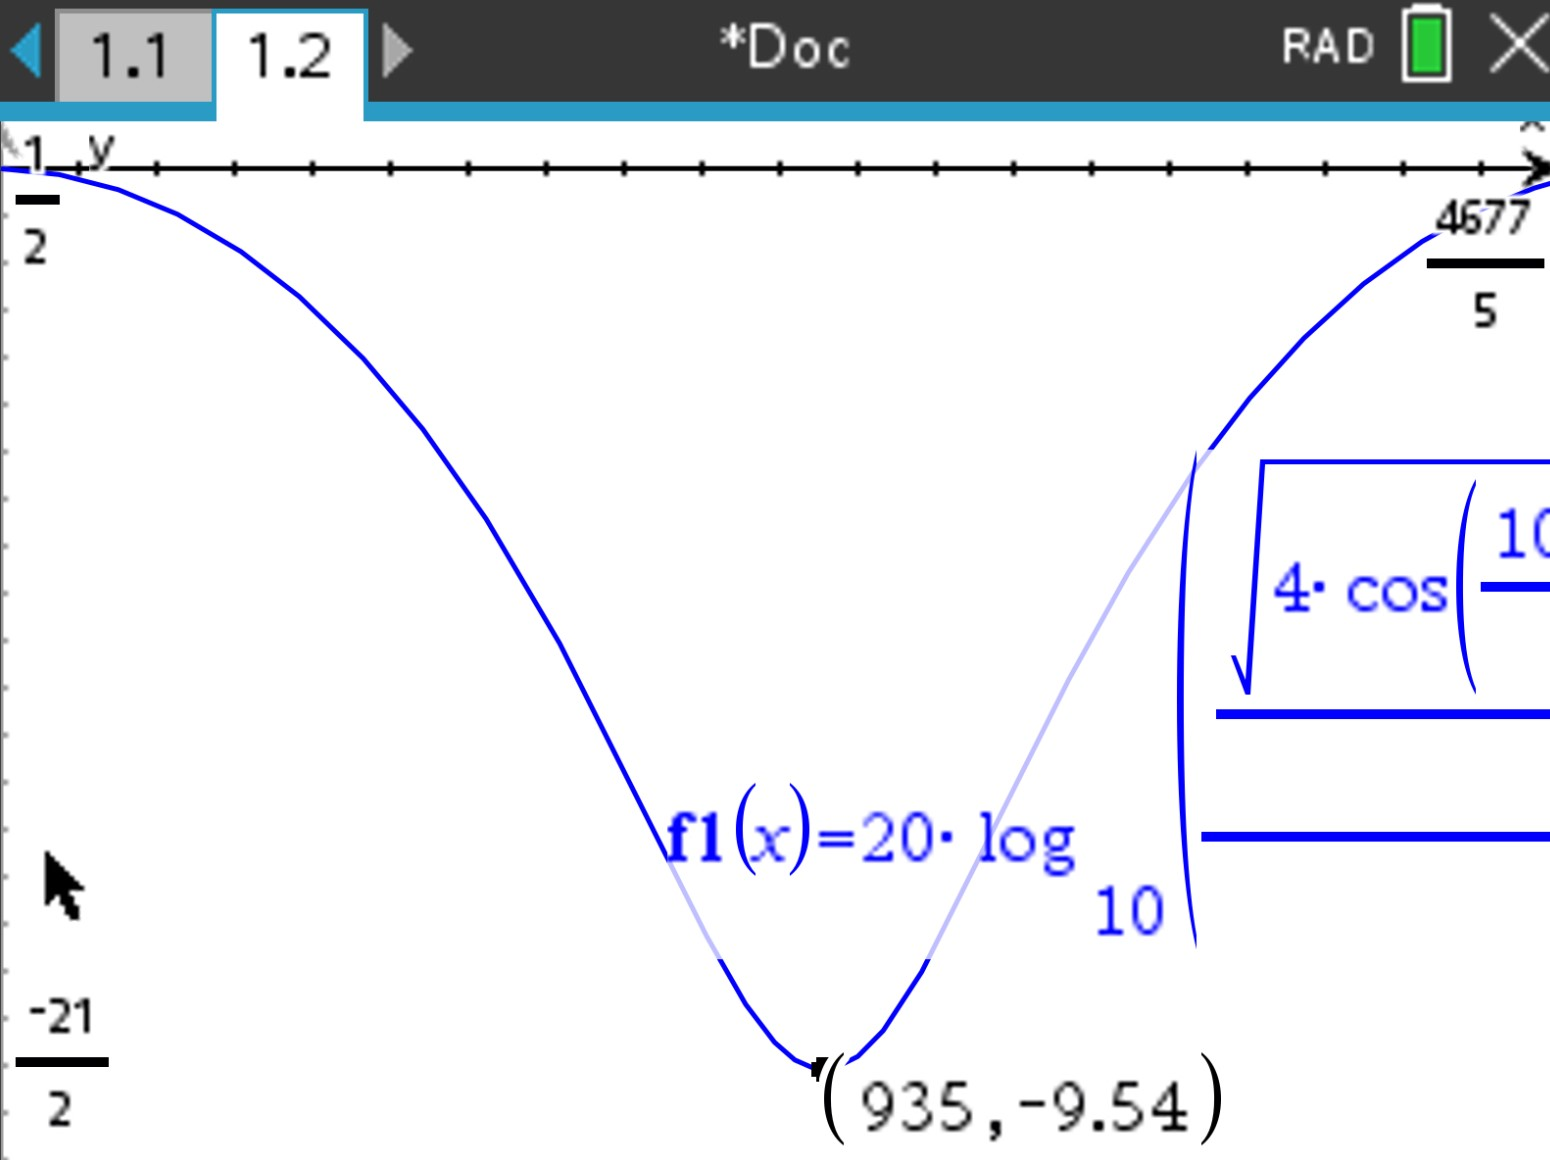
\includegraphics[width=8cm]{images/graph.jpg}
      \caption{plotted graph form exercise}
      \label{fig:graph_ploted}
    \end{figure}
    \item \textbf{Assuming that the radio channel's allowed tolerance of the amplitude response is given by 3dB. Is the radio channel frequency-selective?}\newline
    The radio channel's amplitude response varies up to approximately 10 db as it can also be seen in \autoref{fig:graph_ploted} and is therefore frequency-selective.
    \item \textbf{How will $|\underline{H}(\mathrm{f})|$ change, if the reflection coefficient is changed from 0.5 to 0.8?} \newline
    The reflected path has an increased amplitude. If it is dephased by 180 degrees, the amplitude of the total received signal is more attenuated. Therefore, stronger variations are expected.
    \item\textbf{ In the last example, ' $\textcolor{orange}{r}$ ' was real valued. This is not necessarily the case. How will $|\underline{H}(\mathrm{f})|$ change if the reflection coefficient is given by $\underline{r}_1=0.8 \angle 60^{\circ}$ ?}\newline
    The relative phase relation between direct path and reflected path has been changed. Therefore, the 180 degree out-of-phase occurs at an other frequency. (spectrum is shifted)
    \item \textbf{Consider qualitatively how $|\underline{H}(\mathrm{f})|$ will be changed, if the distance to the mountain chain becomes bigger.}\newline
    The bigger the distance to the mountain, the bigger is the detour $\Delta$. As easily can be seen form the formula for y(f). The relative phase change at a given frequency change is proportional to the detour $\Delta$. It is therefore expected that the amplitude variations with respect to the frequency chances will become faster.
    \item \textbf{The distance to the mountain wall is now given by $h_1$=700m, the reflection coefficient is r=0.5 (real). Is the radio channel-as defined in b) -frequency-selective?}\newline
    No the variations are only about 0.5dB. Since we are closer to the mountain, the periodicity of the channel is lower, as described before.

\end{itemize}
\paragraph{Free-space attenuation}
\begin{itemize}
    \item \textbf{Calculate the free-space attenuation at between two locations at a distance of d= 5km, if the frequency is 900 MHz?}\newline
    According to \autoref{eq:free_space_loss} which says $A_F=(4 \pi \cdot d / \lambda)^2$ one gets $A_F=(4 \pi \cdot \SI{5000}{\meter} / \frac{\SI{3e8}{\meter\per\second}}{\SI{900e6}{\per\second}})^2=\SI{35.53e9}{}$ and in dB: $10\log_{10}(\SI{35.53e9}{})=\SI{105.512}{}$dB
    \item \textbf{What is the rms value of the electrical field at the receiver, if the transmitting power is P=500 W EIRP?}\newline
    According to \autoref{eq:electrical_filed_strength} the following holds $E=\sqrt{\frac{P \cdot G_T \cdot Z_f}{4 \pi d^2}}=\sqrt{\frac{\SI{500}{\watt} \cdot 1 \cdot \SI{377}{\ohm}}{4 \pi (\SI{5000}{\meter})^2}}=\SI{24.4949e-3}{\volt\per\meter}$
\end{itemize}

\paragraph{Okumura-Hata model}
\begin{itemize}
    \item\textbf{ Determine the path loss in urban environment using the Okumura-Hata model for the following scenario:}
    \begin{itemize}
        \item Height of transmitting antenna: $h_t$ = 50m
        \item Height of receiving antenna: $h_r$ = 1.5m
        \item Frequency: f= 900MHz
        \item Distance between transmitter and receiver: d = 5km
        \item Big city
    \end{itemize}
    According to \autoref{eq:okumura-hata} one knows that 
    $$
    \begin{aligned}
    L_{H u}[d B]&=69.55+26.16 \cdot \log \frac{f}{M H z}-13.82 \cdot \log \frac{h_{B S}}{m}-\underbrace{a\left(h_{M S}\right)}_{\text{0 for urban}}+\left(44.9-6.55 \log \frac{h_{B S}}{m}\right) \cdot \log \frac{d}{k m}\\
    &=69.55+26.16 \cdot \log(900) -13.82 \cdot \log(\SI{50}{\meter})+\left(44.9-6.55 \log(\SI{50}{\meter})\right) \cdot \log 5\\&=\underline{\underline{146.959dB}}
    \end{aligned}
    $$
    \item Same scenario, but for rural environment
    $$
    L_{H r}[d B]=146.959dB -4.78 \cdot\left[ \log(900)\right]^2+18.33 \cdot \log(900)-40.94=\underline{\underline{118.452dB}}
    $$
    
    \item Compare the results with result of Problem 2 a)
\end{itemize}
\paragraph{Time-variant channel modelling I}
\begin{itemize}
    \item \textbf{Derive a channel model for a ionospheric 2-path propagation, if the relative time shift between the two signal paths is 1ms whereas the signal bandwidth is 10 kHz.}\newline
    Time resolution is $\frac{1}{W}=\frac{1}{\SI{10}{\kilo\hertz}}=\SI{0.1}{\milli\second}$. ==> The delay line model consists of 10 taps where only the first and the last have (time-varying coefficients)
    \item \textbf{Determine the coherence bandwidth}\newline
    % According to \autoref{eq:corherence_time} the following holds: $\mathrm{T}_{\mathrm{tc}}=1 / \mathrm{B_d}=\frac{1}{}$
    According to \autoref{eq:coherence_bandwidth} the following holds: $\mathrm{B}_{\mathrm{cb}}=1 / \mathrm{T_m}=\frac{1}{\SI{1}{\milli\second}}=\SI{1000}{\hertz}$. Within this bandwidth all frequency components of a signal are modified in a similar way, e.g. all frequency components within $B_c$ could be simultaneously attenuated.
\end{itemize}

\paragraph{Time-variant channel modelling II}
\begin{itemize}
    \item \textbf{Determine a channel model for a communication link between two aircrafts if there is a direct path and a second path resulting from scattering at the earth surface. The scattered path has a delay of $\tau=\SI{10e-6}{\second}$. The signal bandwidth is W=100 kHz.}
    
    \item \textbf{Same scenario, but with a signal bandwidth of W=10kHz}
\end{itemize}


Exam: Bring laptop with to the exam, submission is online, when we write on papaer, we have to scan in programms on the computer are not allowed but local pdfs are.